\begin{title}[\Large]
  Дифференциальное уравнение первого порядка. Основные понятия. Геометрический
  смысл уравнения первого порядка
\end{title}

\begin{define}[обыкновенного дифференциального уравнения]
  ОДУ называется

  $F(x, y(x), y'(x), \ldots, y^{(m)} (x)) = 0$ или

  $F(x, y(x), dx, dy, d^2 x, d^2 y, \ldots d^n x, d^n y) = 0$
\end{define}

\begin{define}[порядка уравнения]
  Порядком уравнения называется максимальный порядок производной или
  дифференциала входящего в уравнение.
\end{define}

\begin{define}[решения ДУ]
  Решение ДУ называется функция

  1) определенная на $<a,b>$

  2) дифференциируема столько раз каков порядок уравнения на $<a,b>$

  3) при подстановке в уравнение обращает его в тождество
\end{define}

\begin{block}[ДУ 1 порядка]
  $F(x, y(x), y'(x)) = 0$ или $F(x, y(x), dy, dx) = 0$

  $y'(x) = f(x, y(x))$ уравнение разрешенное относительно производной. Тоже
  что $\frac{dy(x)}{dx} = f(x, y(x))$

  $f(x, y)$ заданая функция с двумя независимыми переменными. Будем считать
  что эта функция определена и непрерывна в некоторой односвязной области $D$.
\end{block}

\begin{define}[решения ДУ 1 порядка]
  $\varphi (x)$ называется решением уравнения $y'(x) = f(x, y(x))$ если

  1) $\varphi (x)$ определена на $<a,b>$

  2) $\varphi (x)$ диференциируема на $<a,b>$

  3) $\forall x \in <a,b> ~~ \frac{d\varphi (x)}{dx} = f(x, \varphi(x))$

  4) $\forall x \in <a,b> ~~ (x, \varphi(x)) \in D$

  График решения называется интегральной кривой
\end{define}

\begin{define}[задачи Коши]
  Задачей Коши для $y'(x) = f(x, y(x))$ называется
  решение уравнения которое при заданом $x_0$ принимает
  заданное значение $y_0$ то есть $y(x_0) = y_0$
  называется условие Коши или начальное условие
  $$
  \left\{
  \begin{array}{l}
    y'(x) = f(x, y(x)) \\
    y(x_0) = y_0
  \end{array}
  \right.
  $$
\end{define}

\begin{define}[общего решния ДУ]
  Общим решением уравнения $y'(x) = f(x, y(x))$ называется $y = y(x,C)$
  такая что $\forall C$ функция является решением уравнения и любое
  решение уравнения входит в это семейство при некоторых $C$.

  Решение при конкретном $C$ называется частным решением.
\end{define}

\begin{define}[изоклина]
  $y' = f(x,y)$

  $y'(x) = \tg \alpha$

  $\tg \alpha = f(x,y)$

  $\tg \alpha = A$

  $f(x, y) = A$ изоклин

  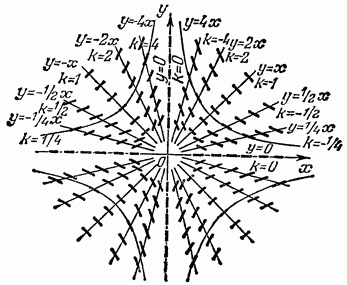
\includegraphics[width = 9cm]{izoklin}
\end{define}

\begin{block}[Интегральный тип уравнений]
  $$
  y'(x) = f(x) ~~~ y(x) = \int f(x)dx + C
  $$
  $y(x_0) = y_0$ задача Коши
  $$
  \left( \int_{x_0}^x f(t) dt \right)' = f(x) ~~~ \int f(x)dx = \int_{x_0}^x
  f(t)dt + C
  $$
  $$
  y(x) = \int_{x_0}^x f(t)dt + C ~ \text{общее решение}
  $$
  $$
  y(x) = \int_{x_0}^x f(t)dt + y_0 ~ \text{решение задачи Коши}
  $$
\end{block}

\begin{title}[\Large]
  Уравнения с разделяющимися переменными (определение, нахождение решения)
\end{title}

\begin{define}[уравнения с разделяющимися переменными]
  Уравнения с разделяющимися переменными (УРП) называют
  $$
  y'(x) = f(x) \cdot g(y(x))
  $$
  $$
  \frac{dy(x)}{dx} = f(x) \cdot g(y(x))
  $$
\end{define}

\begin{block}[Общий вид решения УРП]
  $$
  \frac{dy(x)}{dx} = f(x) \cdot g(y(x))
  $$
  $$
  \int \frac{dy(x)}{g(y(x))} = \int f(x)dx ~~~ g(y(x)) \not= 0
  $$
  $$
  \int \frac{dy(x)}{g(y(x))} = \int f(x)dx
  $$
  $$
  F'(x) = f(x) ~~~ G'(u) = \frac{1}{g(u)}
  $$
  $$
  G(y(x)) = F(x) + C
  $$
\end{block}

\begin{title}[\Large]
  Теорема существования и единственности решения задачи Коши для уравнения с
  разделяющимися переменными
\end{title}

\begin{theorem}[о $\exists !$ решения УРП]
  $f(x), g(u)$ определены и непрерывны на $x \in <a, b> ~ u \in <c, d>$
  $g(u) \not= 0$ тогда
  $\forall x_0 \in <a, b> ~~~ \forall y_0 \in <c, d>$
  $$
  \exists!
  \left\{
  \begin{array}{l}
    y'(x) = f(x) g(y(x)) \\
    y(x_0) = y_0
  \end{array}
  \right.
  $$
  Замечание: $\exists m \in <c, d> ~ g(m) = 0$ тогда $y(x) \equiv m$
\end{theorem}

\begin{proof}
  1) Докажем единственность. Предположим что $\varphi(x)$ решение уравнения
  $y'(x) = f(x, y(x))$ удовлетворяющее $y(x_0) = y_0$ то есть
  $\varphi(x_0) = y_0$
  $$
  x \in <a, b> ~~~ \frac{d\varphi(x)}{dx} \equiv f(x)g(\varphi(x))
  $$
  $$
  \frac{d(\varphi(x))}{g(\varphi(x))} \equiv f(x)dx
  $$
  $$
  \int_{x_0}^x \frac{d(\varphi(t))}{g(\varphi(t))} = \int_{x_0}^x f(t)dt
  $$
  $$
  u = \varphi(t) ~~~ \int_{\varphi(x_0)}^{\varphi(x)} \frac{du}{g(u)} =
  \int_{x_0}^x f(t)dt
  $$
  $$
  \int_{y_0}^{\varphi(x)} \frac{du}{g(u)} = \int_{x_0}^x f(t)dt
  $$
  $$
  \text{пусть} ~ F'(t) = f(t) ~~~ G'(u) = \frac{1}{g(u)}
  $$
  $$
  G(u) |_{y_0}^{\varphi(x)} = F(x) - F(x_0)
  $$
  $$
  G(\varphi(x)) = G(y_0) + F(x) - F(x_0)
  $$
  $g(u) \not= 0$

  $g(u)$ сохраняет знак

  $G'(u) = \frac{1}{g(u)}$ сохраняет знак

  $G'(u) \not= 0$

  $G(u)$ строго монотонна и непрерывна $\Rightarrow$
  $\exists$ обратная ей функция
  $$
  \varphi(x) = G^{-1} ( G(y_0) + F(x) + F(x_0))
  $$
  из едеинственности обратной функции $\Rightarrow$ единственность решения

  2) Докажем существование
  $$
  \colorbox[rgb]{0.7,0.7,0}{$(G^{-1}(y))' = \frac{1}{G'(G^{-1}(y))}$}
  $$
  $$
  \varphi'(x) = \frac{1}{G'( G^{-1} (G(y_0) + F(x) + F(x_0))} \cdot
  (G(y_0) + F(x) + F(x_0))' =
  $$
  $$
  = f(x) \cdot g \left( G^{-1} (G(y_0) + F(x) + F(x_0))
  \right) = f(x) \cdot g(\varphi(x))
  $$
  $\Rightarrow ~ \varphi(x)$ решение задачи
\end{proof}

\begin{theorem}
  Если $\int_m \frac{du}{g(u)}$ расходится, то через каждую точку области
  проходит единственное решение

  Если $\int_m \frac{du}{g(u)}$ сходится, то в точках $y = m$ единственность
  нарушена
\end{theorem}

\begin{title}[\Large]
  Уравнения приводящиеся к УРП
\end{title}

\begin{block}[Уравнения сводящиеся к линейной замене]
  $$
  y'(x) = f(\alpha x + \beta y(x) + \gamma) ~~~ \alpha, \beta, \gamma \in R
  $$
  $$
  z(x) = \alpha x + \beta y(x) + \gamma
  $$
  $$
  z'(x) = \alpha + \beta y'(x) ~~~ \beta \not= 0
  $$
  $$
  z'(x) = \beta f(z(x)) + \alpha ~~ \text{тоже что и} ~~
  z'(x) = 1 \cdot g(z(x))
  $$
\end{block}

\begin{block}[Однородные уравнения]
  $$
  y'(x) = \Phi \left( \frac{y(x)}{x} \right) ~~~ z(x) = \frac{y(x)}{x}
  $$
  $$
  y(x) = z(x) \cdot x
  $$
  $$
  y'(x) = z'(x) x + z(x)
  $$
  $$
  \Phi(z(x)) = z'(x)x + z(x)
  $$
  $$
  z'(x) = \frac{\Phi(z(x)) - z(x)}{x}
  $$
\end{block}

\begin{title}[\Large]
  Линейный дифференциальные уравнения 1 порядка. Метод вариации произвольных
  постоянных
\end{title}

\begin{define}[линейного однородного и неоднородного уравнения]
  $y'(x) = a(x)y(x) + b(x)$ линейное неоднородное уравнение

  $y'(x) = a(x)y(x)$ линейное однородное уравнение
\end{define}

\begin{block}[Общее решение линейного однородного уравнения]
  $$
  y'(x) = a(x)y(x)
  $$
  $$
  \frac{dy(x)}{dx} = a(x)y(x)
  $$
  $$
  \int \frac{dy(x)}{y(x)} = \int a(x)dx ~~~ y(x) \not= 0
  $$
  $$
  \ln |y(x)| = \int a(x)dx + C
  $$
  $$
  |y(x)| = e^{\int_{x_0}^x a(t) dt + C}
  $$
  $$
  y(x) = C e^{\int_{x_0}^x a(t) dt}
  $$
\end{block}

\begin{block}[Метод вариации произвольной постоянной]
  $$
  y(x) = C(x) e^{\int_{x_0}^x a(t) dt}
  $$
  найдем $C(x)$ так чтобы $y(x)$ стала решением неоднородного уравнения
  $$
  y'(x) = C'(x) \cdot e^{\int_{x_0}^x a(t) dt} +
  C(x) \cdot \left( e^{\int_{x_0}^x a(t) dt} \right)' =
  $$
  $$
  = C'(x) \cdot e^{\int_{x_0}^x a(t) dt} +
  C(x) \cdot e^{\int_{x_0}^x a(t) dt} a(x)
  $$
  $$
  C'(x) \cdot e^{\int_{x_0}^x a(t) dt} +
  C(x) \cdot e^{\int_{x_0}^x a(t) dt} a(x) =
  a(x) C(x) \cdot e^{\int_{x_0}^x a(t) dt} + b(x)
  $$
  $$
  C'(x) = \frac{b(x)}{e^{\int_{x_0}^x a(t) dt}} =
  b(x) e^{-\int_{x_0}^x a(t) dt}
  $$
  $$
  C(x) = \int_{x_0}^x b(s) e^{-\int_{x_0}^s a(t) dt} ds + D
  $$
  $$
  y(x) = \left( \int_{x_0}^{x} e^{-\int_{x_0}^t a(\tau) d\tau}
  b(t)dt + D \right) \cdot e^{\int_{x_0}^x a(\tau) d\tau} =
  $$
  $$
  = D e^{\int_{x_0}^x a(\tau) d\tau} + \int_{x_0}^x
  e^{\int_{x_0}^x a(\tau) d\tau - \int_{x_0}^t a(\tau) d\tau} b(t)dt
  $$
  $$
  y(x) = D e^{\int_{x_0}^x a(\tau) d\tau} + \int_{x_0}^x
  e^{\int_{t}^x a(\tau) d\tau} b(t)dt
  $$
\end{block}

\begin{title}[\Large]
  Теорема существования и единственности решения задачи Коши для линейного
  уравнения 1 порядка
\end{title}

\begin{block}[Формула Коши]
  $$
  \left\{
  \begin{array}{l}
    y'(x) = a(x)y(x) + b(x) \\
    y(x_0) = y_0
  \end{array}
  \right. ~~~ \text{задача Коши}
  $$
  $$
  y(x) = y_0 e^{\int_{x_0}^x a(\tau) d\tau} + \int_{x_0}^x
  e^{\int_{t}^x a(\tau) d\tau} b(t)dt
  $$
  $$
  K(x, t) = e^{\int_t^x a(\tau) d\tau}
  $$
  $$
  y(x) = y_0 K(x, x_0) + \int_{x_0}^x K(x, t) b(t) dt
  $$
  $K(x, t)$ функция Коши
\end{block}

\begin{block}[Свойства]
  1) $K(x, x) = 1$

  2) при каждом фиксираванном $t \in <\alpha, \beta> ~ K(x, t)$ есть решение
  $y'(x) = a(x)y(x)$
\end{block}

\begin{theorem}
  $a(x), b(x)$ определены и непрерывны на $<\alpha, \beta>$
  тогда задача Коши $\forall x_0 \in <\alpha, \beta> ~~ \forall y_0 \in R$
  $\exists !$ решение которое выражается
  $$
  y(x) = y_0 e^{\int_{x_0}^x a(\tau) d\tau} + \int_{x_0}^x
  e^{\int_{t}^x a(\tau) d\tau} b(t)dt
  $$
\end{theorem}

\begin{proof}
  1) Докажем единственность решения. Предположим что есть другое решение задачи
  Коши тогда
  $$
  \varphi(x) = u(x) e^{\int_{x_0}^x a(\tau)d\tau}
  $$
  проделов те же действия что и в методе вариаций получим что
  $\varphi(x) = y(x)$.

  2) Докажем существование.
  $$
  \left( \int_{\alpha(x)}^{\beta(x)} F(x, t) dt \right)' =
  F(x, \beta(x)) \beta'(x) - F(x, \alpha(x)) \alpha'(x) +
  \int_{\alpha(x)}^{\beta(x)} F_x(x, t)dt
  $$
  $$
  y'(x) = y_0 e^{\int_{x_0}^x a(\tau) d\tau} a(x) + \left( \int_{x_0}^x
  e^{-\int_{x_0}^t a(\tau) d\tau} b(t)dt \cdot
  e^{\int_{x_0}^x a(\tau)d\tau} \right)' =
  $$
  $$
  = y_0 e^{\int_{x_0}^x a(\tau)d\tau} a(x) + b(x)
  e^{-\int_{x_0}^x a(\tau) d\tau} \cdot e^{\int_{x_0}^x a(\tau) d\tau} +
  $$
  $$
  + \int_{x_0}^x e^{-\int_{x_0}^t a(\tau) d\tau} b(t) dt \cdot
  e^{\int_{x_0}^x a(\tau) d\tau} \cdot a(x)=
  $$
  $$
  = a(x) \left( y_0 e^{\int_{x_0}^x a(\tau) d\tau} + \int_{x_0}^x b(t)
  e^{\int_t^x a(\tau) d\tau} dt \right) + b(x) =
  $$
  $$
  = a(x)y(x) + b(x)
  $$
\end{proof}

\begin{title}[\Large]
  Уравнение Бернули
\end{title}

\begin{block}[Уравнение Бернули]
  $$
  y'(x) = a(x)y(x) + b(x)y^m(x) ~~~ m \not= 0 \not= 1
  $$
  $$
  \frac{y'(x)}{y^m(x)} = a(x) y^{1 - m}(x) + b(x)
  $$
  $$
  z(x) = y^{1 - m}(x)
  $$
  $$
  z'(x) = (1 - m) y^{-m}(x) y'(x) = \frac{(1-m)y'(x)}{y^m(x)}
  $$
  $$
  \frac{y'(x)}{y^m(x)} = \frac{z'(x)}{1 - m}
  $$
  $$
  z'(x) = (1 - m) a(x)z(x) + (1 - m)b(x)
  $$
\end{block}

\begin{title}[\Large]
  Уравнение в полных дифференциалах(определение, нахождение решения)
\end{title}

\begin{define}[уравнения в полных дифференциалах]
  Уравнение вида $P(x, y)dx + Q(x, y)dy = 0$ называется, уравнением в полных
  дифференциалах, если $\exists F(x, y)$
  $$
  \left\{
  \begin{array}{l}
    \frac{\partial F(x, y)}{\partial x} = P(x, y) \\
    \frac{\partial F(x, y)}{\partial y} = Q(x, y)
  \end{array}
  \right.
  $$
  $$
  \frac{\partial P(x, y)}{\partial y} = \frac{\partial Q(x, y)}{\partial x}
  $$
  $dF(x, y) = 0 ~ \Rightarrow ~ F(x, y) \equiv C$ 1-ый интеграл уравнения.

  Если частные производные 2-ого порядка существуют и непрерывны, то они равны
  $\frac{\partial^2 F}{\partial x \partial y} =
  \frac{\partial^2 F}{\partial y \partial x}$
\end{define}

\begin{block}[Решение уравнений в полых дифференциалах в общем виде]
  начальное условие $(x_0, y_0)$
  $$
  F(x, y) = \int_{x_0}^x P(t, y)dt + C(y)
  $$
  $$
  \frac{\partial F(x, y)}{\partial y} =
  \left( \int_{x_0}^x P(t, y)dt + C(y) \right)'_y =
  \int_{x_0}^x \frac{\partial P(t, y)}{\partial y} dt + C'(y) =
  $$
  $$
  = \int_{x_0}^x \frac{\partial Q(t, y)}{\partial t} dt + C'(y) =
  Q(t, y)|_{x_0}^x + C'(y) = Q(x, y) - Q(x_0, y) + C'(y) = Q(x, y)
  $$
  $$
  C'(y) = Q(x_0, y)
  $$
  $$
  C(y) = \int_{y_0}^y Q(x_0, t) dt + D
  $$
  $$
  F(x, y) = \int_{x_0}^x P(t, y) + \int_{y_0}^y Q(x_0, t) dt + D
  $$
  $$
  \int_{x_0}^x P(t, y)dt + \int_{y_0}^y Q(x_0, t) dt = C
  $$
\end{block}

\begin{theorem}
  $$
  \left\{
  \begin{array}{l}
    P(x,y)dx + Q(x,y)dy = 0 \\
    F(x_0, y_0) = 0
  \end{array}
  \right. ~ \text{задача Коши}
  $$
  $P(x, y), Q(x, y)$ непрерывны в некоторой односвязной области $G$ и
  $\forall (x,y) \in G ~~ Q(x, y) \not= 0$ и существуют непрерывные частные
  производные, тогда $\forall (x_0, y_0) \in G$ задача Коши
  $\exists !$ решение.
\end{theorem}